\model{File Search}

Recursion is typically not used to implement functions like \java{factorial} and \java{summation}; those examples were only meant to demonstrate how recursive methods work.
A more common use of recursion is searching for files on your computer.
The following Linux command recursively searches for a file named \java{week1.txt}:

\vspace{1em}
\java{\$ find -name week1.txt}
\vspace{1em}

Note that \$ represents the command-line prompt; it's not part of the command itself.


\quest{10 min}


\Q What are the two arguments of the \texttt{find} command in \ref{\currfilename}?
Why do you think the first argument is necessary?

\begin{answer}
The first argument \texttt{-name} indicates we are searching for a file by name, as opposed to by type or by size. The second argument \texttt{week1.txt} is the name of the file to find.
\end{answer}


\Q Consider the following files and directories.
What is the absolute path of \texttt{week1.txt}?

\begin{center}
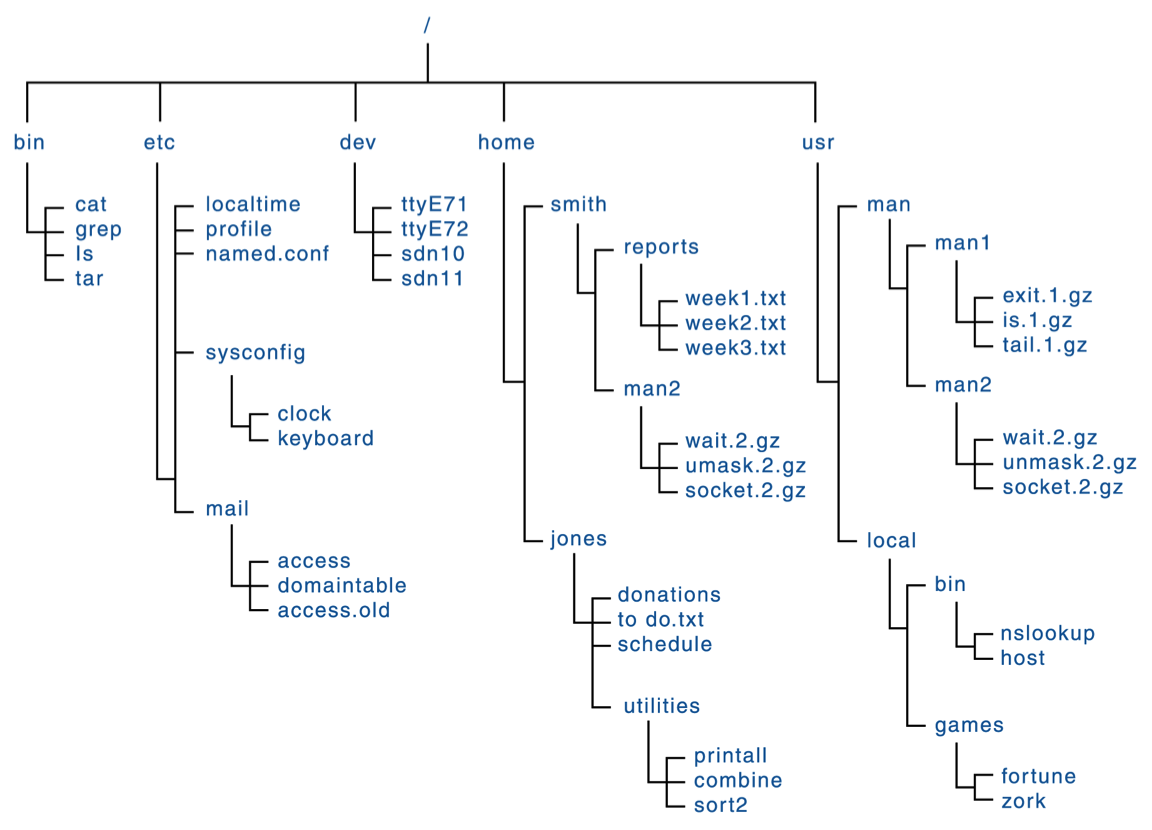
\includegraphics[height=4in]{files-unix.png}
\end{center}


\Q Describe an algorithm (in simple English) for finding files on your computer.
Use phrases like ``for each directory'' and ''for each file''.

\begin{answer}
// list the current directory
// check the name of each file
// search each sub directory
// base case: file not found
\end{answer}


\Q Outline a recursive method in Java to search for files.
You don't need to write the exact code, but show the recursive step.

\begin{javalst}
public static final File find(File rootDir, String fileName) {












}
\end{javalst}
